\subsection{Entwurf eines browserbasierten GUI}\label{l:entwurf-gui}

Das browserbasierte GUI der Anwendung ist der wichtigste Zugang zum System, da es von allen Mitarbeiter zu irgendeinem Zeitpunkt verwendet wird. Die Zeit, die der Einzelne damit verbringt kann sich je nach Rolle stark unterscheiden. Neben den sehr unterschiedlichen Anforderungen and das GUI sind die Benutzer auch technisch sehr unterschiedlich stark versiert, wie in den Personas in Kapitel \ref{l:personas} · S.\pageref{l:personas} gezeigt wurde. Diesen Umständen muss bei der Gestaltung eines GUI Rechnung getragen werden. In Anlehnung an \cite{nielsen} wurden für den Entwurf der browserbasierten GUI folgende Leitlinien gewählt:

\begin{enumerate}\itemsep -5pt
\item{Das wichtigste zuerst: Die aktuelle Aufgabe soll immer im Fokus der Darstellung liegen.}
\item{Schnell zum Ziel: Alle Aufgaben müssen leicht und umkompliziert durchführbar sein.}
\item{Nicht ablenken: Veränderungen in der Darstellung, z.B. durch Benachrichtigungen, lenken ab und müssen deswegen so gestaltet sein, dass diese sich nach den Präferenzen des Nutzers richten.}
\item{Hilfe nur einen Klick entfernt: Das Hilfesystem muss kontextsensitiv verfügbar sein und ist eine Kernfunktion der Anwendung}
\end{enumerate}

Da die Anwendung von allen Benutzern gerne verwendet werden soll und vor allem die Usability und die Zeitersparnis ein wichtiger Punkt sind, wie man auch skeptische Mitarbeiter überzeugen kann, mit ihren alten Gewohnheiten zu brechen, ist die Beachtung dieser Grundsätze essentiell. Funktionalitäten, die nur von wenigen gebraucht werden, sollten, wenn überhaupt, optional einblendbar sein. Die Konzeption des Systems ermöglicht es leicht, zusätzliche Anwendungen für besondere Benutzergruppen zu schaffen, z.B. Plug-Ins für die speziellen Werkzeuge einzelner Mitarbeiter. Für diese \typoquotes{Power-User} ist dieser Weg meistens der bessere Weg.

\begin{table}
\begin{center}
\begin{tabular}{@{}l c c c c c c c}
& \textbf{Eva} & \textbf{Lotte} & \textbf{Torsten} &  \textbf{Jorinde} & \textbf{Jan} & \textbf{Arthur} & \textbf{Markus}\\
{\small Operation (vgl.~\ref{l:workflow})} & {\small Konz.} & {\small Des.} & {\small Texter} & {\small Übersetz.} & {\small Prod.} & {\small Projektl.} & {\small Kunde}\\
\hline\\[-1.5ex]
Definieren         & \HarveyFull      & \HarveyQuarter   & \HarveyEmpty    & \HarveyEmpty    & \HarveyEmpty   & \HarveyEmpty     & \HarveyEmpty \\
Schreiben          & \HarveyQuarter   & \HarveyEmpty     & \HarveyFull     & \HarveyFull     & \HarveyEmpty   & \HarveyEmpty     & \HarveyEmpty \\
Korrektur          & \HarveyEmpty     & \HarveyEmpty     & \HarveyHalf     & \HarveyHalf     & \HarveyEmpty   & \HarveyQuarter   & \HarveyQuarter \\
Qualitätskontrolle & \HarveyQuarter   & \HarveyEmpty     & \HarveyEmpty    & \HarveyEmpty    & \HarveyEmpty   & \HarveyFull      & \HarveyHalf \\
Freigabe           & \HarveyEmpty     & \HarveyEmpty     & \HarveyEmpty    & \HarveyEmpty    & \HarveyEmpty   & \HarveyQuarter   & \HarveyQuarter \\
Veröffentlichung   & \HarveyEmpty     & \HarveyEmpty     & \HarveyEmpty    & \HarveyEmpty    & \HarveyQuarter & \HarveyEmpty     & \HarveyEmpty \\
\end{tabular}
\caption{Umfang und Häufigkeit der Benutzung des browserbasierten GUIs bezogen auf die durchgeführten Operation}
\label{table:webgui-usage-by-persona}
\end{center}
\end{table}

Anhand der Personas lässt sich ermitteln, wer und in welchem Umfang das browserbasiert GUI verwenden wird. Tabelle \ref{table:webgui-usage-by-persona} · S.\pageref{table:webgui-usage-by-persona} zeigt in der Übersicht, welche Operationen besonders bei der Entwicklung des GUIs beachtet werden müssen. Besonders viel Zeit werden von Konzeptern und von den Mitarbeiter, die die Inhalte Erstellen, Kontrollieren und Freigeben im GUI verbracht, da diese Tätigkeiten bezogen auf die einzelnen Texte des Produktes sehr arbeitsintensiv sind.

\bigskip

Die folgenden Wireframes zeigend dementsprechend die wichtigsten Ansichten des GUIs.

\subsubsection{Aufbau des GUIs}\label{l:gui-aufbau}

\begin{center}
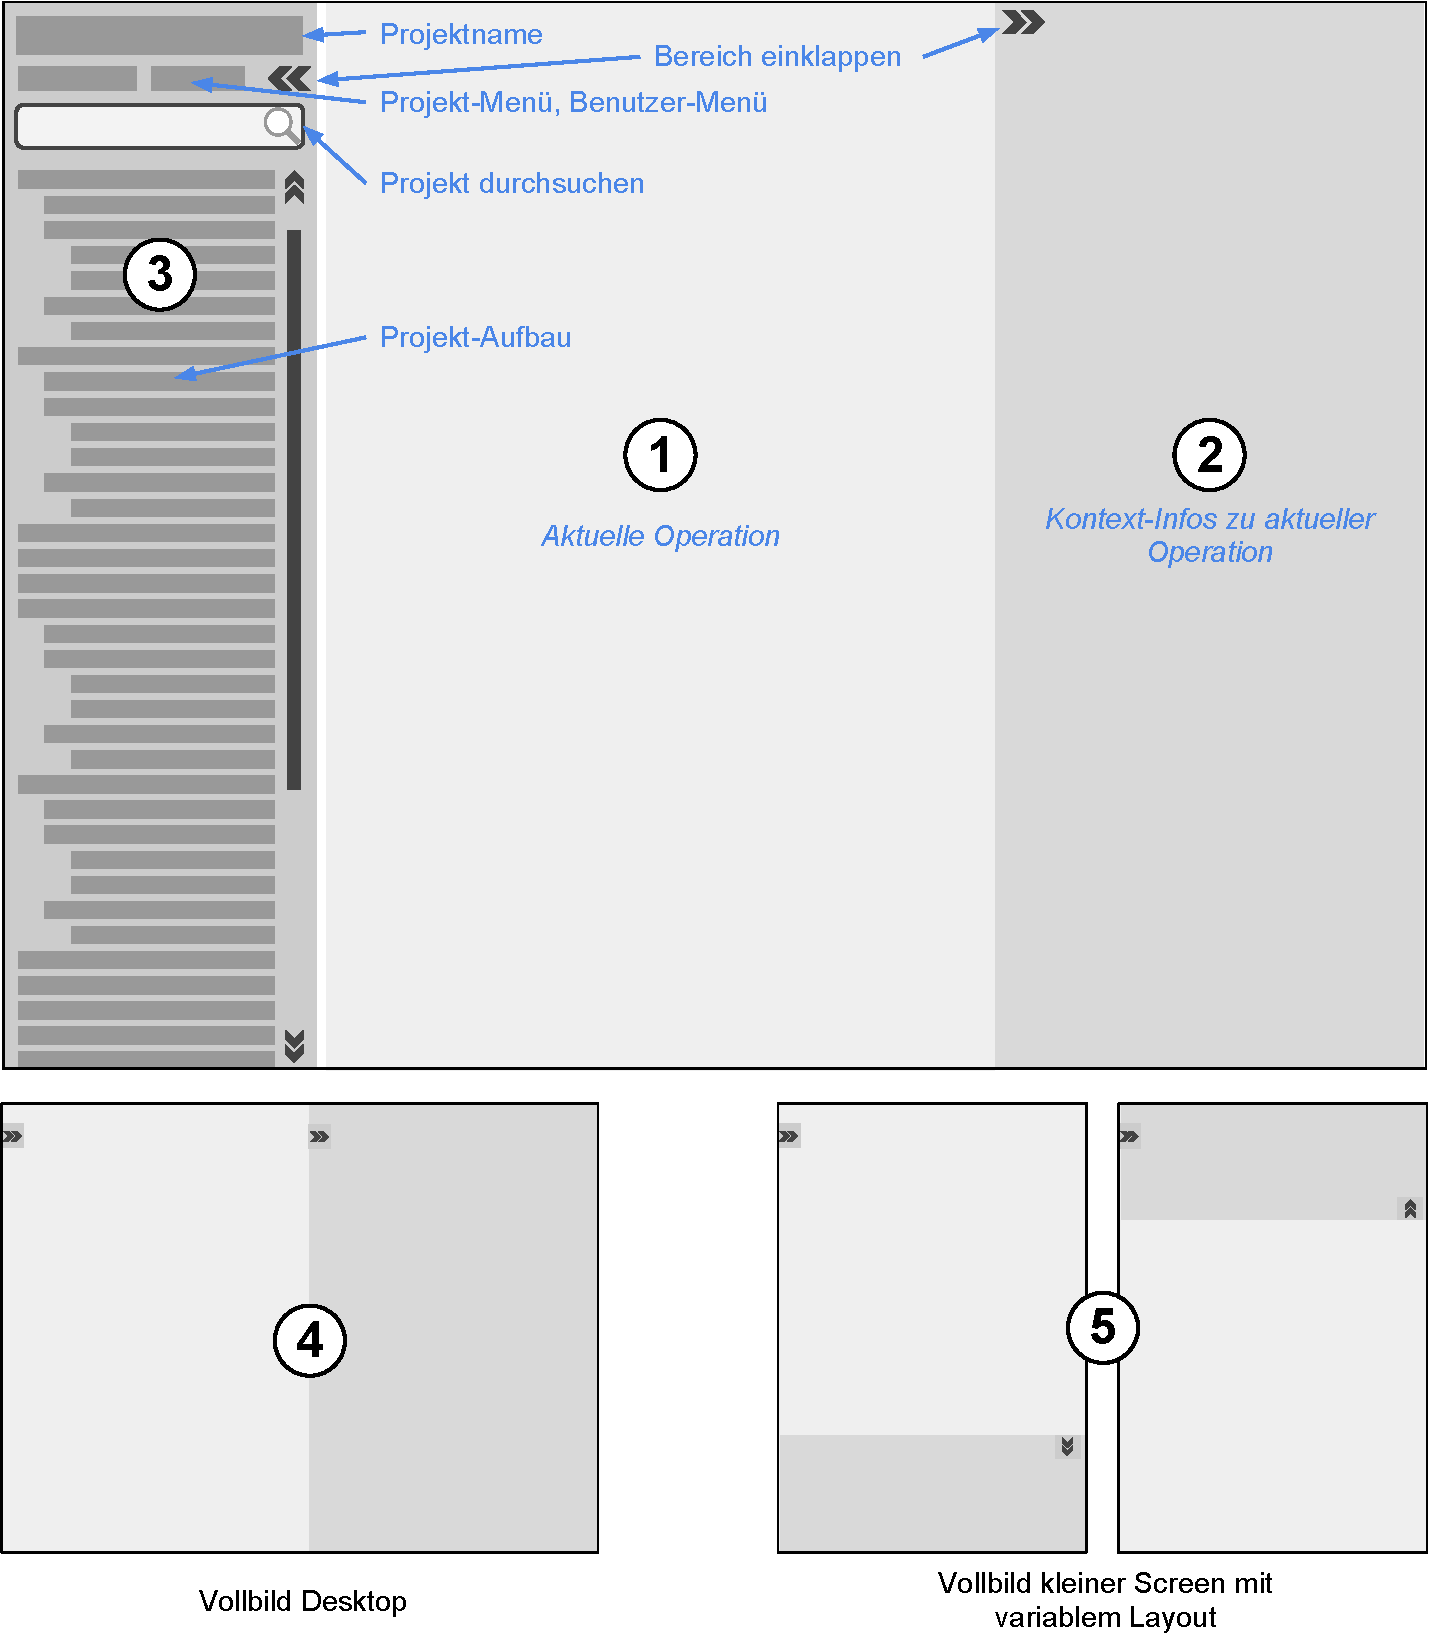
\includegraphics[width=0.95\textwidth]{media/GUIAufbau.pdf}
\captionof{figure}{Aufbau des browserbasierten GUIs}\label{chart:gui-aufbau}
\end{center}

Abbildung~\ref{chart:gui-aufbau} zeigt den Grundaufbau des GUIs. Zentraler Bereich ist die Darstellung der \emph{aktuellen Operation} \ball{1} mit den zugehörigen \emph{Kontext-Informationen} \ball{2}. Auf der linke Seite findet sich eine Spalte über die im Projekt navigiert werden kann \ball{3}. Um den Fokus auf die aktuelle Aufgaben zu verbessern sind die Kontext-Information und die Projektspalte ausblendbar \ball{4}. Das gesamte Layout passt sich flexibel an verschiedene Bildschirmgrößen und -formate an, zusätzlich kann die Position der Kontext-Information an die eigenen Vorlieben angepasst werden \ball{5}.

Die Projekt-Spalte \ball{3} bietet direkten Zugang zu allen Teilen des aktiven Projekts. Die Projektstruktur wird mit einem Navigationsbaum dargestellt, über den direkt zu den jeweiligen Abschnitten gesprungen werden kann. Über das Suchfeld lässen sich die Einträge im Baum filtern. In der Spalte befindet sich oben zur Orientierung der Names des aktiven Projektes. Über das ausklappbare Projektmenü gelangt man Teilen der Anwendung, die nicht direkt über die Texte erreichbar sind, z.B. Projektauswahl, Mitarbeiterverwaltung, Export. Über das ausklappbare Benutzermenü kann man sich ausloggen, sein Profil bearbeiten und persönliche Einstellungen anpassen.

\subsubsection{Definieren des Produktes}\label{l:gui-definition}

\begin{center}
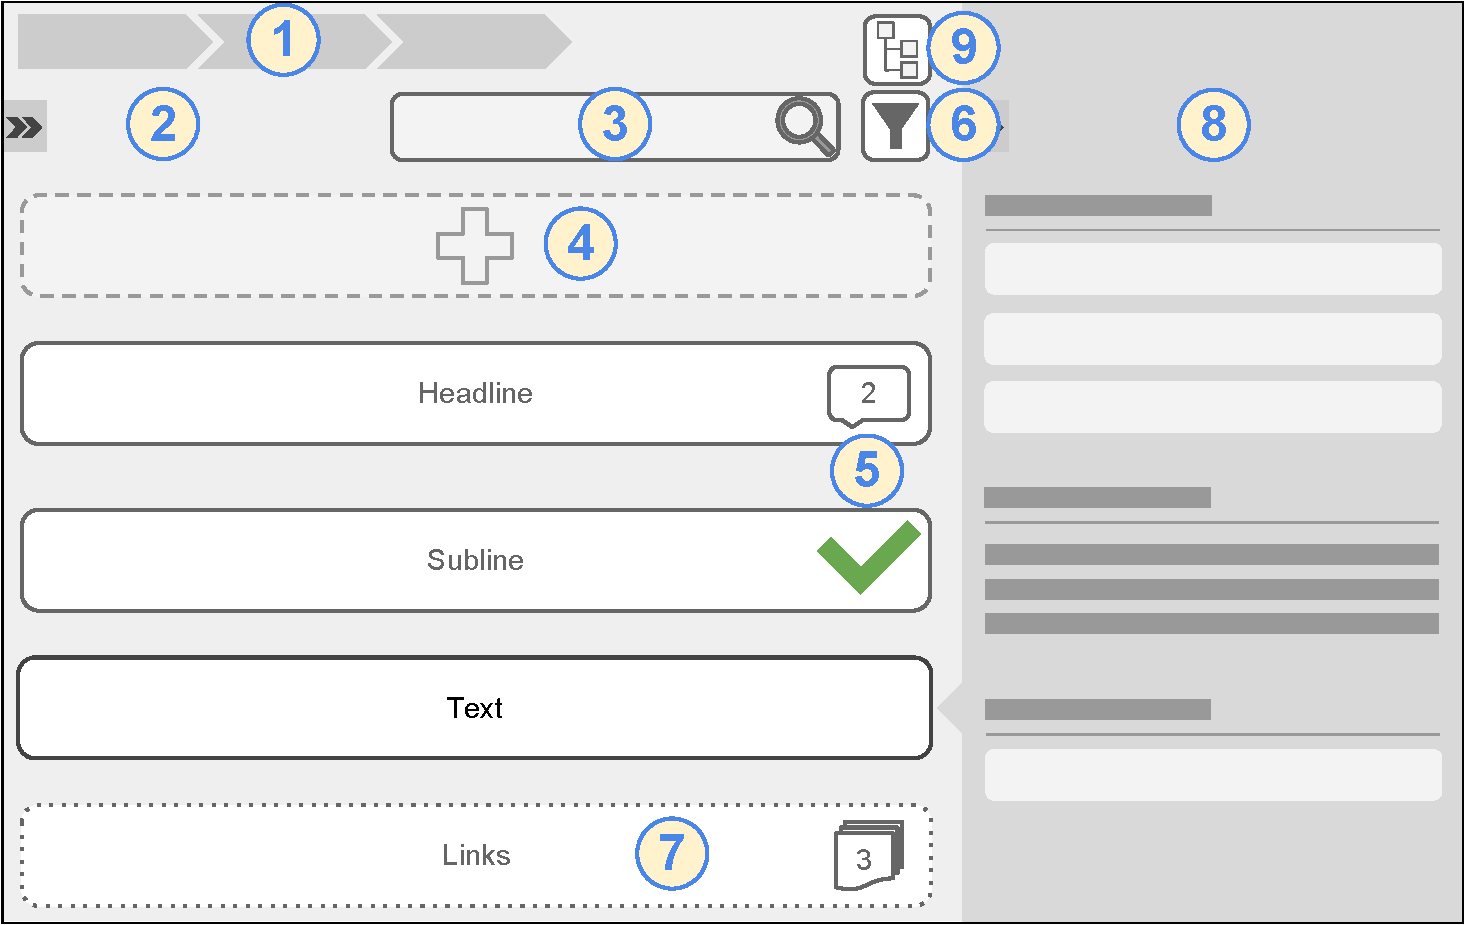
\includegraphics[width=0.95\textwidth]{media/GUIProduktstruktur.pdf}
\captionof{figure}{GUI zum Bearbeiten der Produktstruktur}\label{chart:gui-produktstruktur}
\end{center}

Abbildung~\ref{chart:gui-produktstruktur} zeigt die Darstellung des GUIs zur Bearbeitung der Produktstruktur. Über die Breadcrumb-Navigation \ball{1}, die die aktuelle Position in der Projekthierarchie zeigt, ist eine Orientierung auch ohne das eingeklappte Projektmenü möglich. Über eine Schaltfläche lassen sich alle Container aber der aktuellen Hierarchiebene aufklappen, so ist können umfangreiche Änderungen an vielen Elementen gleichzeitig vorgenommen werden, ohne dass man sich durch die verschiedenen Ebenen \typoquotes{hangeln} muss. Im Inhaltsbereich \ball{2} werden die auf der aktuellen Ebene befindlichen Inhalts-Elemente, Textbausteine und Container, angezeigt. Die Darstellung erfolgt in eine kompakten Weise, die einen schnellen Überblick über die Inhalte bietet ohne viel Scrollen zu müssen. Die einzelnen Inhalts-Elemente können mit Drag\&Drop in ihrere Reihenfolge angepasst werden. Über das Suchfeld \ball{3} können die angezeigten Elemente gefiltert werden. Über eine Schaltfläche \ball{4} können neue Inhalts-Elemente erstellt werden. Zusatzinformationen wie der Typ, der Status, Kommentare oder ähnliche können auch verwendet werden, um die Inhalte auf der Seite zu filtern, z.B. um nur die Element anzuzeigen, für die noch die Inhalte fehlen \ball{5}. Durch Klick auf einen Container \ball{6} gelangt man eine Ebene tiefer, in diesen Conatiner hinein. Das Icon gibt die Anzahl der untergeordneten Element an. In der Spalte für die Kontext-Information \ball{7} werden Detailinformation zum aktuell ausgewählten Element dargestellt, die an die eingestellten Ansichts-Art angepasst sind. Hier findet sich auch die Bearbeitungshistorie und die Kommentare zu den Inhalts-Elementen.

Über eine Schaltfläche \ball{8} kann zwischen den vier Ansichten (Definieren~\ref{l:gui-definition}, Texten~\ref{l:gui-texten}, Übersetzen~\ref{l:gui-uebersetzen} und Kontrolle~\ref{l:gui-qs}), die die Inhaltselemente manipulieren, gewechselt werden.

\subsubsection{Texte erstellen}\label{l:gui-texten}

\begin{center}
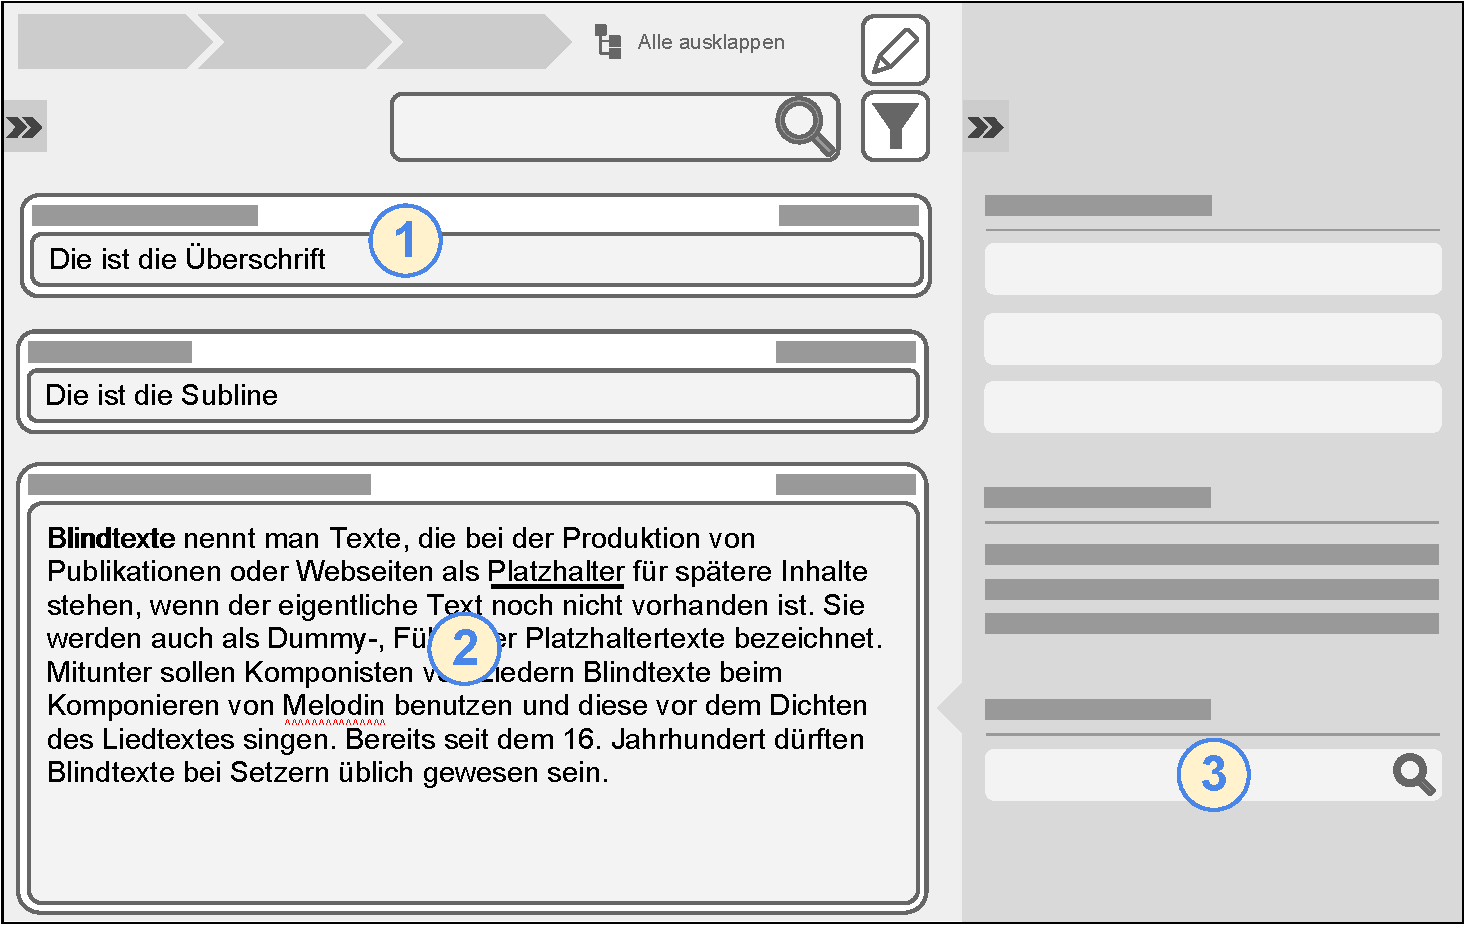
\includegraphics[width=0.95\textwidth]{media/GUITexteerstellen.pdf}
\captionof{figure}{GUI zum Erstellen der Texte}\label{chart:gui-texten}
\end{center}

Abbildung~\ref{chart:gui-texten} zeigt die Darstellung des GUIs zur Bearbeitung der Texte des Produktes. Die Inhaltselemente in der aktuelle Hierarchie werden dabei mit Eingabefeldern für die Inhalte dargestellt \ball{1}. Links über dem Eingabefeld wird die Bezeichnung des Textbausteins angezeigt und rechts darüber Hinweise zu Längebeschränkungen (falls vorhanden) mit Zähler. Während der Eingabe können bereits Auszeichnungen vorgenommen werden, die Schaltflächen dazu, werden eingeblendet, sobald sich der Cursor im Feld befindet. Innerhalb der Kontext-Informationen \ball{3} besteht die Möglichkeit direkt eine Suche zu starten, die Suchergebnisse werden in einem Dialog-Fenster geöffnet. 

\subsubsection{Texte übersetzen}\label{l:gui-uebersetzen}

\begin{center}
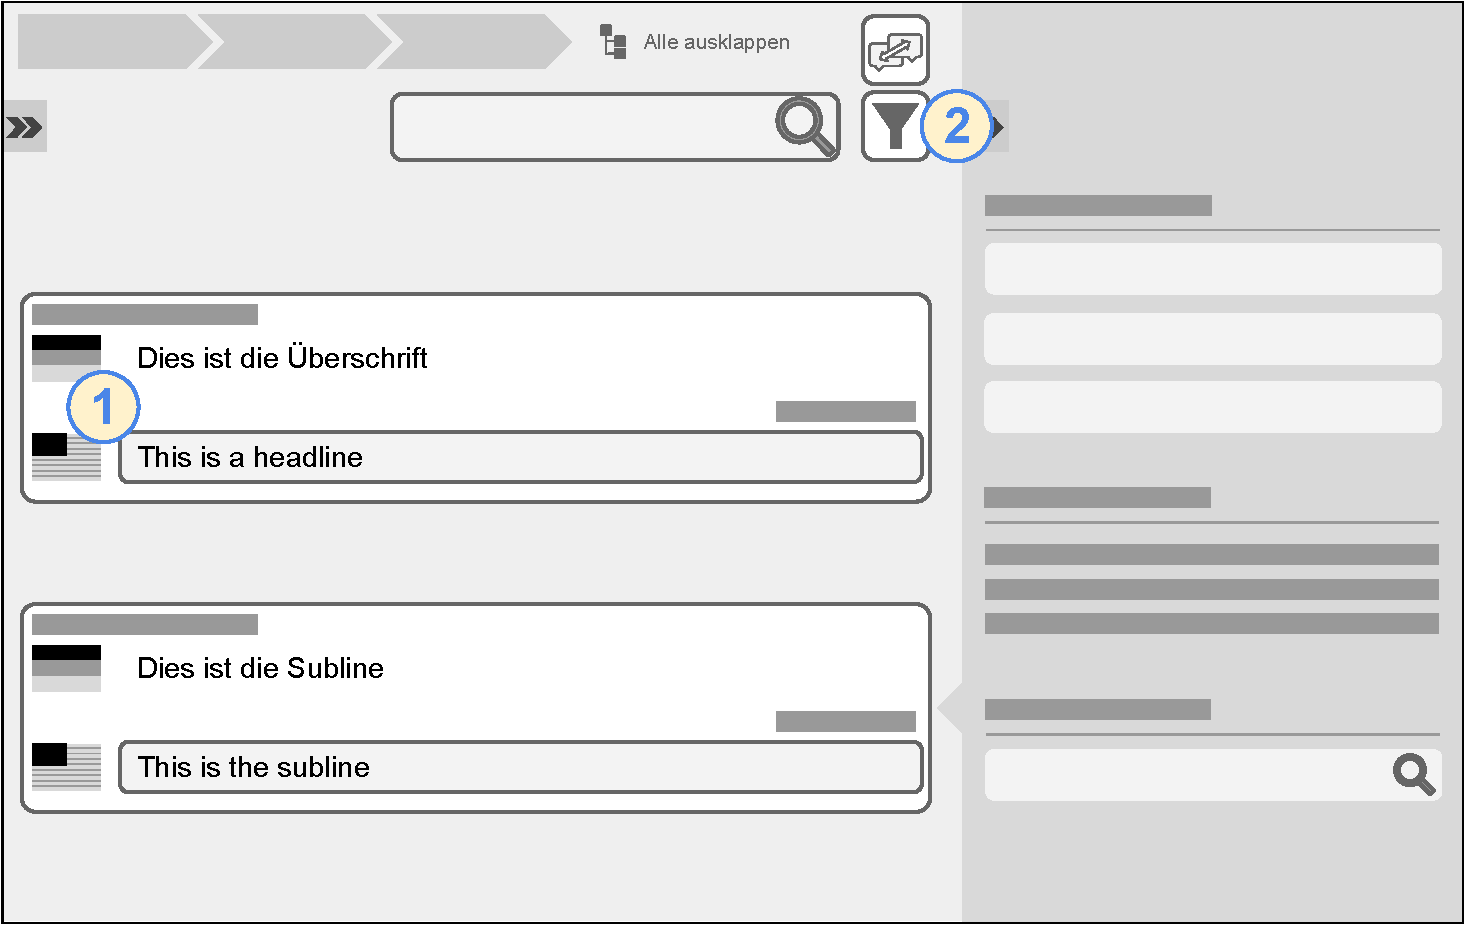
\includegraphics[width=0.95\textwidth]{media/GUITexteuebersetzen.pdf}
\captionof{figure}{GUI zum Übersetzen der Texte}\label{chart:gui-uebersetzen}
\end{center}

Abbildung~\ref{chart:gui-uebersetzen} zeigt die Darstellung des GUIs zur Übersetzung der Texte des Produktes. Hierzu wird der Inhalt des Textbausteines in der Original-Sprache angezeigt und darunter ein Eingabefeld, in dem die Übersetzung eingetragen wird \ball{1}. Über einen Filter-Dialog \ball{2} kann konfiguriert werden, welche Sprachen angezeigt werden sollen.

\subsubsection{Prüfen}\label{l:gui-qs}

\begin{center}
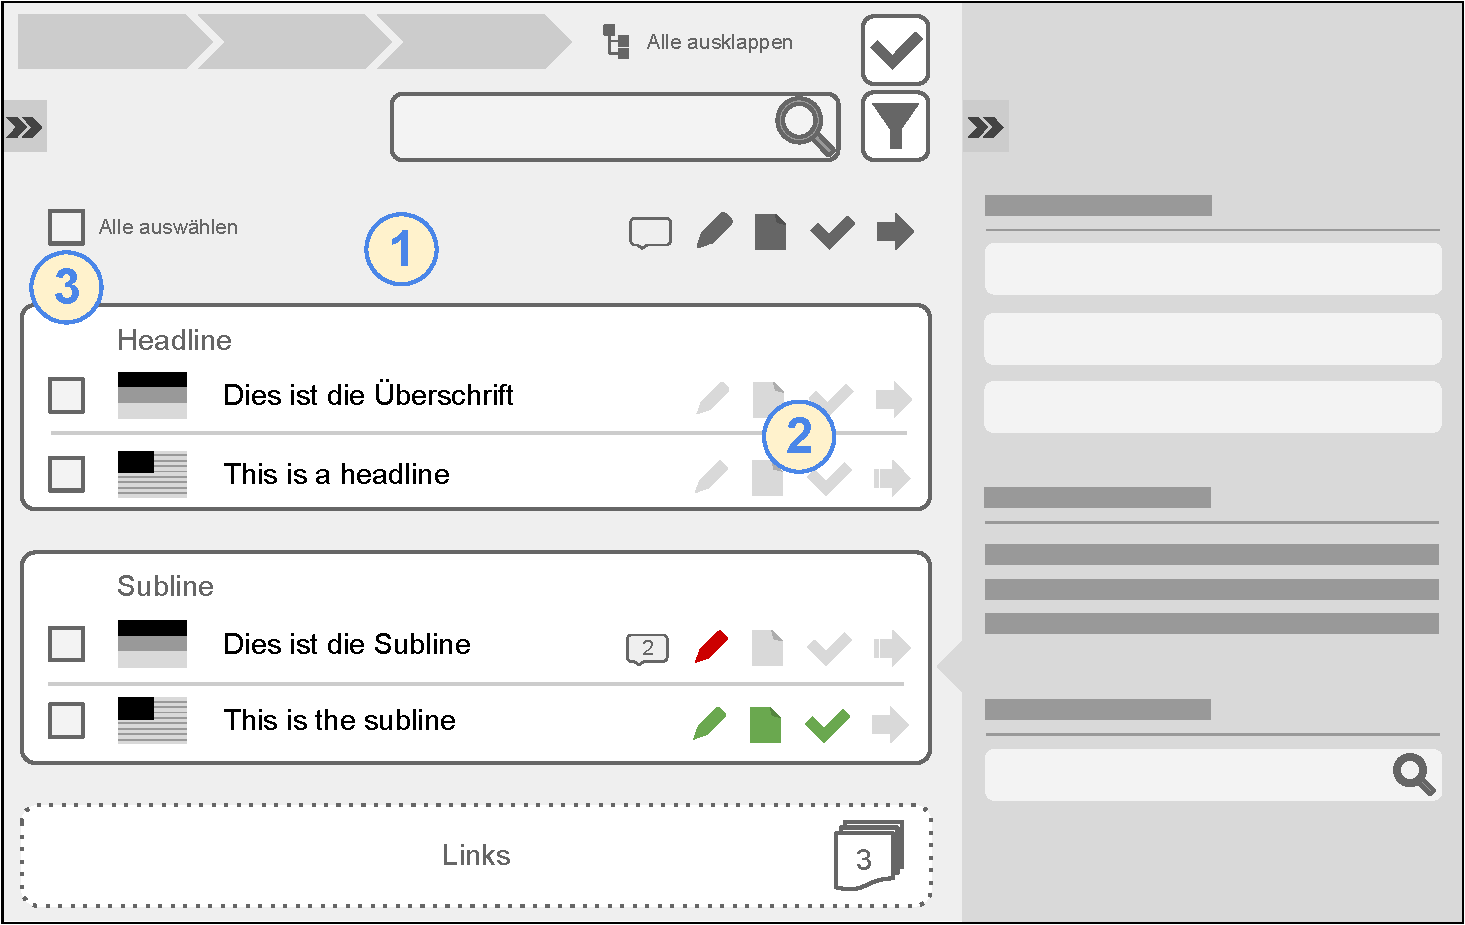
\includegraphics[width=0.95\textwidth]{media/GUIFreigabe.pdf}
\captionof{figure}{GUI zum Überprüfen der Texte}\label{chart:gui-qs}
\end{center}

Abbildung~\ref{chart:gui-qs} zeigt die Darstellung des GUIs zur Kontrolle und Freigabe der Texte des Produktes. In dieser Ansicht werden die verschiedenen Stati der Textbausteine bearbeitet. Hierzu sind die Textbausteine mit ihren Übersetzungen dargestellt \ball{1}. Über die mit Icons markierten Schaltflächen \ball{2} lassen sich die einzelnen Stati direkt setzen. Von links nach rechts sind das: Korrigiert, Geprüft, Freigegeben und Veröffentlicht. Es wird jeweils zwischen \typoquotes{keine Angabe} (grau), \typoquotes{abgelehnt} (rot) und \typoquotes{in Ordnung} (grün) unterschieden. Hier wird auch die Anzahl der hinterlegten Kommentare angezeigt. Zum massenhaften bearbeiten von Stati können mehrere oder alle Elemente über die Checkboxen \ball{3} ausgewählt werden. Über die Status-Icons in der Kopfzeile kann dann der Status für alle ausgewählten Elemente gleichzeitig gesetzt werden.

\subsubsection{Kontext-Informationen}\label{l:gui-kontext}

\begin{center}
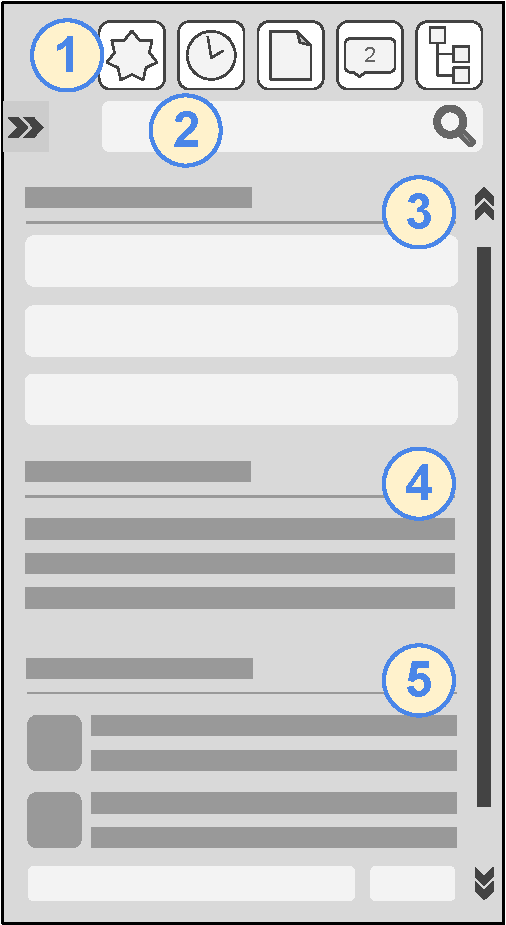
\includegraphics[width=0.35\textwidth]{media/GUIKontext-Informationen.pdf}
\captionof{figure}{Kontext-Informationen}\label{chart:gui-kontext}
\end{center}

Abbildung~\ref{chart:gui-kontext} zeigt die Darstellung des GUIs zur Anzeige und Bearbeitung der Kontext-Informationen. Der Inhalt der Ansicht ist an die jeweilige Operation angepasst. Im oberen Bereich kann zwischen verschiedenen Kontextinformationen zu dem jeweiligen Inhalt umgeschaltet werden \ball{1} (v.l.n.r): 

\begin{enumerate}\itemsep -5pt
\item Neues: Listet die neuesten Informationen aus den vier Bereichen und den aktuellen Status.
\item Änderungshistorie: Zeigt die vergangenen Änderungen an, mit der Möglichkeit, diese zu kommentieren und zurückzunehmen.
\item Material: Zeigt hinterlegte Materialien an. Dabei handelt es sich um Dateien und Freitext-Notizen.
\item Kommentare: Zeigt die Kommentare an.
\item Struktur: Zeigt Informationen zur Struktur innerhalb des Produktes, wie z.B. die Attribute, an.
\end{enumerate}

Über das Suchfeld \ball{2} lässt sich die aktuellen Ansicht filtern. In den Kontextinformation findet sich direkter Zugang zu Informationen und Operationen bezogen auf den aktuellen Inhalt. Die Inhalte lassen sich über Formulare \ball{3} direkt bearbeiten, Notizen und Dateien werden angezeigt \ball{4} und der Diksussion mithilfe der Kommentarfunktion ist möglich \ball{5}.

\secbar

Die in diesem Abschnitt gezeigten Wireframes sind die Vorlage für eine mögliche Implementierung. Bei der Umsetzung des Protypen wurde versucht, dieser Vorlage weitestgehend zu folgen, wie in Abschnitt \ref{l:implementierung-gui} · S.\pageref{l:implementierung-gui} beschrieben wird. Im nächsten Abschnitt wird jedoch zuerst auf die Verbindung des Anwendungsservers mit einem GUI eingegangen.